% iaus2esa.tex -- sample pages for Proceedings IAU Symposium document class
% (based on v1.0 cca2esam.tex)
% v1.04 released 17 May 2004 by TechBooks
%% small changes and additions made by KAvdH/IAU 4 June 2004
% Copyright (2004) International Astronomical Union

\NeedsTeXFormat{LaTeX2e}

\documentclass{iau_FM}
\usepackage{graphicx}

\title[Physics of Common Envelopes] %% give here short title %%
{Powering and Shaping Planetary Nebulae: The Physics of Common Envelopes}

\author[Nordhaus \& Spiegel]   %% give here short author list %%
{Jason Nordhaus$^{1,2}$, David S. Spiegel$^3$}


\affiliation{$^1$Dept. of Science and Mathematics, National Technical Institute for the Deaf\\
Rochester Institute of Technology, Rochester, NY 14623, USA  \\[\affilskip]
$^2$Center for Computational Relativity and Gravitation\\
Rochester Institute of Technology, Rochester, NY 14623, USA\\ email: {\tt nordhaus@astro.rit.edu}\\[\affilskip]
$^3$Algorithms Department, Stitch Fix\\
San Francisco, CA 94103, USA}

\pubyear{2015}
\setcounter{page}{1}
\jname{Astronomy in Focus, Volume 1} 
\editors{Piero Benvenuti, ed.}
\begin{document}

\maketitle

\begin{abstract}
The diversity of collimated outflows in post-asymptotic-giant-branch stars and their planetary nebula progeny are often explained by a combination of close binary interactions and accretion.  The viability of such scenarios can be tested by comparing  kinematic outflow data to determine minimum accretion rates necessary to power observed outflows.  While many binary channels have been ruled out with this technique, common envelope interactions can accommodate the current observational constraints, are potentially common, lead to a diverse array of planetary-nebula shapes, and naturally produce period gaps for companions to white dwarfs.
\keywords{stars: AGB and post-AGB
, (stars:) binaries (including multiple): close, stars: magnetic fields, stars: mass loss, (stars:) planetary systems, stars: evolution}
\end{abstract}

\firstsection % if your document starts with a section,
              % remove some space above using this command.
\section{Introduction}

For stars with initial masses $\lesssim$~8$M_\odot$, post-main-sequence evolution is accompanied by significant expansion of the stellar radius and copious mass loss during the giant phases. As the stellar envelope depletes, a natal white dwarf (WD) emerges encased in an optically-dark reflection nebula.  Subsequent heating by the WD ionizes the expanding-stellar material which shines as a planetary nebulae (PN).  Originally, the ejected nebulae were thought to be spherical and originate from steady mass loss by an isolated star during the Asymptotic Giant Branch (AGB) phase. However, this paradigm changed as high-resolution-optical imaging revealed highly anisotropic and collimated structures such as jets, disks and fast-clumpy ejecta (\cite{BF2002,DeMarco2009,Z2015}).

The transition from spherical mass loss during the AGB phase to the collimated and magnetized outflows seen in the post-AGB and PN phases is thought to arise in systems with close binary companions (\cite{2006MNRAS.370.2004N,DeMarco2009}).  The diversity of observed outflows and their kinematic properties are often explained by various combinations of binary interactions and accretion with the most energetic interactions occurring when the orbital separation decays to short periods ($\lesssim 1$ day) (\cite{2006MNRAS.370.2004N,2007MNRAS.376..599N}).  Companions initially orbiting within $\sim$5-8 AU during the main sequence are expected to plunge into their host stars during the RGB or AGB phases (\cite{NS2013}).  Once immersed in such common envelopes, the companion inspirals until it ejects the giant's envelope, emerging in a post-CE short-period orbit, or is destroyed (\cite{spiegel2012}).

Here, we highlight recent work relevant to common envelopes (CEs) including (i.) how outflow observations in post-AGB/PN can be used to constrain engine-driving scenarios, (ii.) how stellar evolution leads to period gaps for companions to white dwarfs and (iii.) how highly-magnetized white dwarfs can form in common envelopes.


\section{Viable Binary Channels}
The observational challenges inherent in detecting post-AGB star binaries and planetary nebulae binaries have led many to study indirect constraints expected from the presence, or absence, of companions.  Kinematic observations of the large-scale outflows can provide constraints on engine-driving scenarios based on measurements of momentum and energy in the outflows.  For example, using the kinetic energy of jets and tori in a sample of post-AGB stars, \cite{2012IAUS..283..188H} found that their sum was greater than the binding energy of the progenitor envelope.

Recently, \cite{BL2014} used observations of outflow momenta from the same sample to calculate the minimum necessary accretion rates to power the outflows.  These rates were then compared to theoretical models to obtain minimum accretion rates needed for each scenario under the assumption that all accreted power goes into the outflows.  The authors considered two accretors, a main-sequence star and a white dwarf, and four accretion paradigms, Bondi-Hoyle-Littleton (BHL) wind accretion, Roche-lobe overflow at the rate measured for the Red Rectangle, accretion during a common envelope phase and Wind-Roche-lobe overflow.  Various modes of accretion could then be ruled out for the 19 systems considered in their sample.  


\begin{figure}[b]
% \vspace*{-2.0 cm}
\begin{center}
 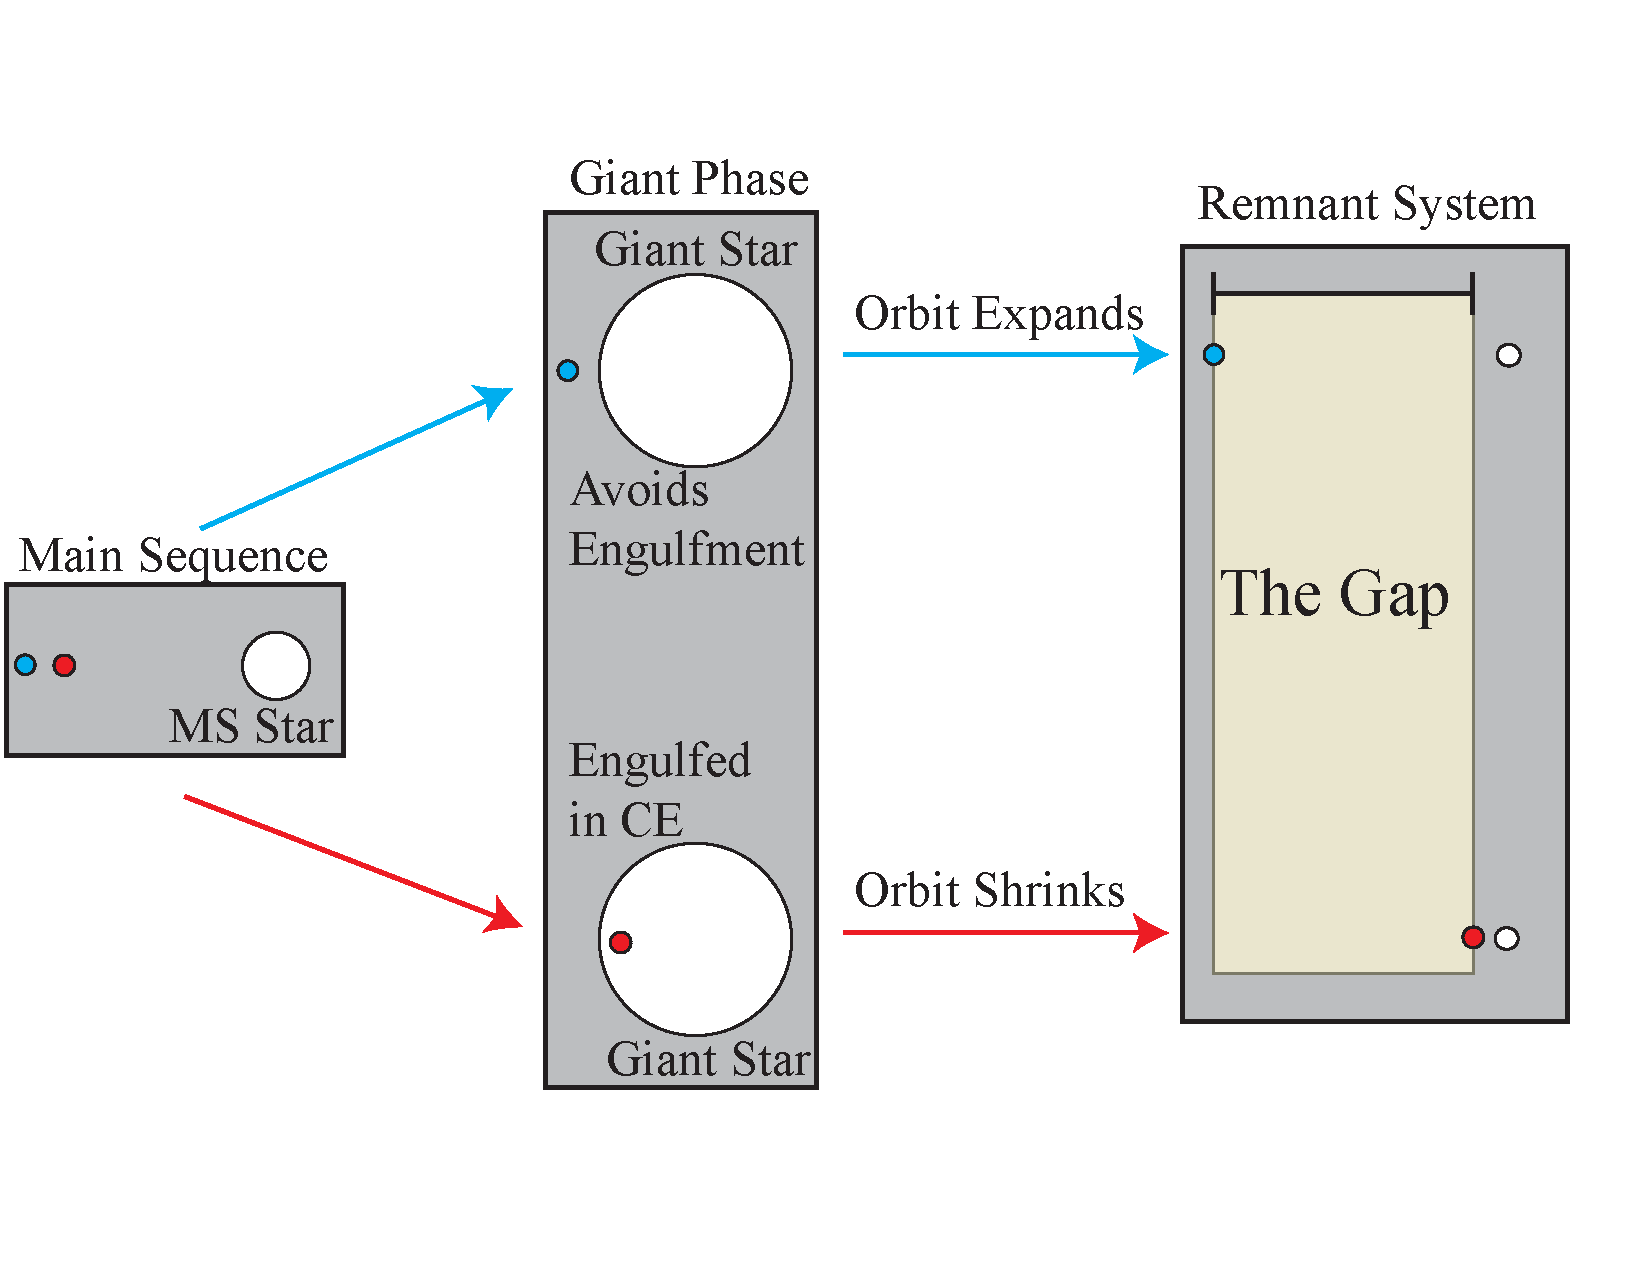
\includegraphics[width=5in]{GapFigure.pdf} 
% \vspace*{-1.0 cm}
 \caption{Post-main-sequence evolution naturally leads to period gaps for companions to white dwarfs (\cite{NS2013}).  The blue companion avoids engulfment during the giant phases and migrates outward as mass is lost from the system.  The red companion's orbit shrinks as it is engulfed in a common envelope and emerges in a short-period orbit around the WD.  As a result, a paucity of companions to white dwarfs are predicted for orbital periods in ``The Gap".}
   \label{fig1}
\end{center}
\end{figure}

Bondi-Hoyle-Littleton wind accretion and Wind-Roche-lobe overflow were ruled out as explanations for the vast majority of objects.  Roche-lobe overflow at the rate measured in the Red Rectangle could accommodate $\sim$1/3 of the objects.  The only paradigm that successfully powers all objects was accretion during a common envelope phase.  Note this does not imply that common envelopes power these systems, only that there is the necessary power available in CE events to explain the observed outflows.


\section{Common Envelopes}

Since companions to main-sequence stars are plentiful, it may be that common envelopes are in fact common events as stars evolve off the main-sequence.  When a companion is engulfed in a common envelope, rapid inspiral on short timescales leads to a sharp reduction in separation between the companion and the giants core (\cite{1976IAUS...73...75P}).  Energy and angular momentum are transferred from the orbit to the CE itself during this process and can be used to unbind the envelope.  Thus, common envelopes represent one method of shrinking a binary's separation from initial periods on the order of years to final periods on the order of hours.  Here, we detail two additional areas in which common envelopes are thought to be important.

\begin{figure}[b]
% \vspace*{-2.0 cm}
\begin{center}
 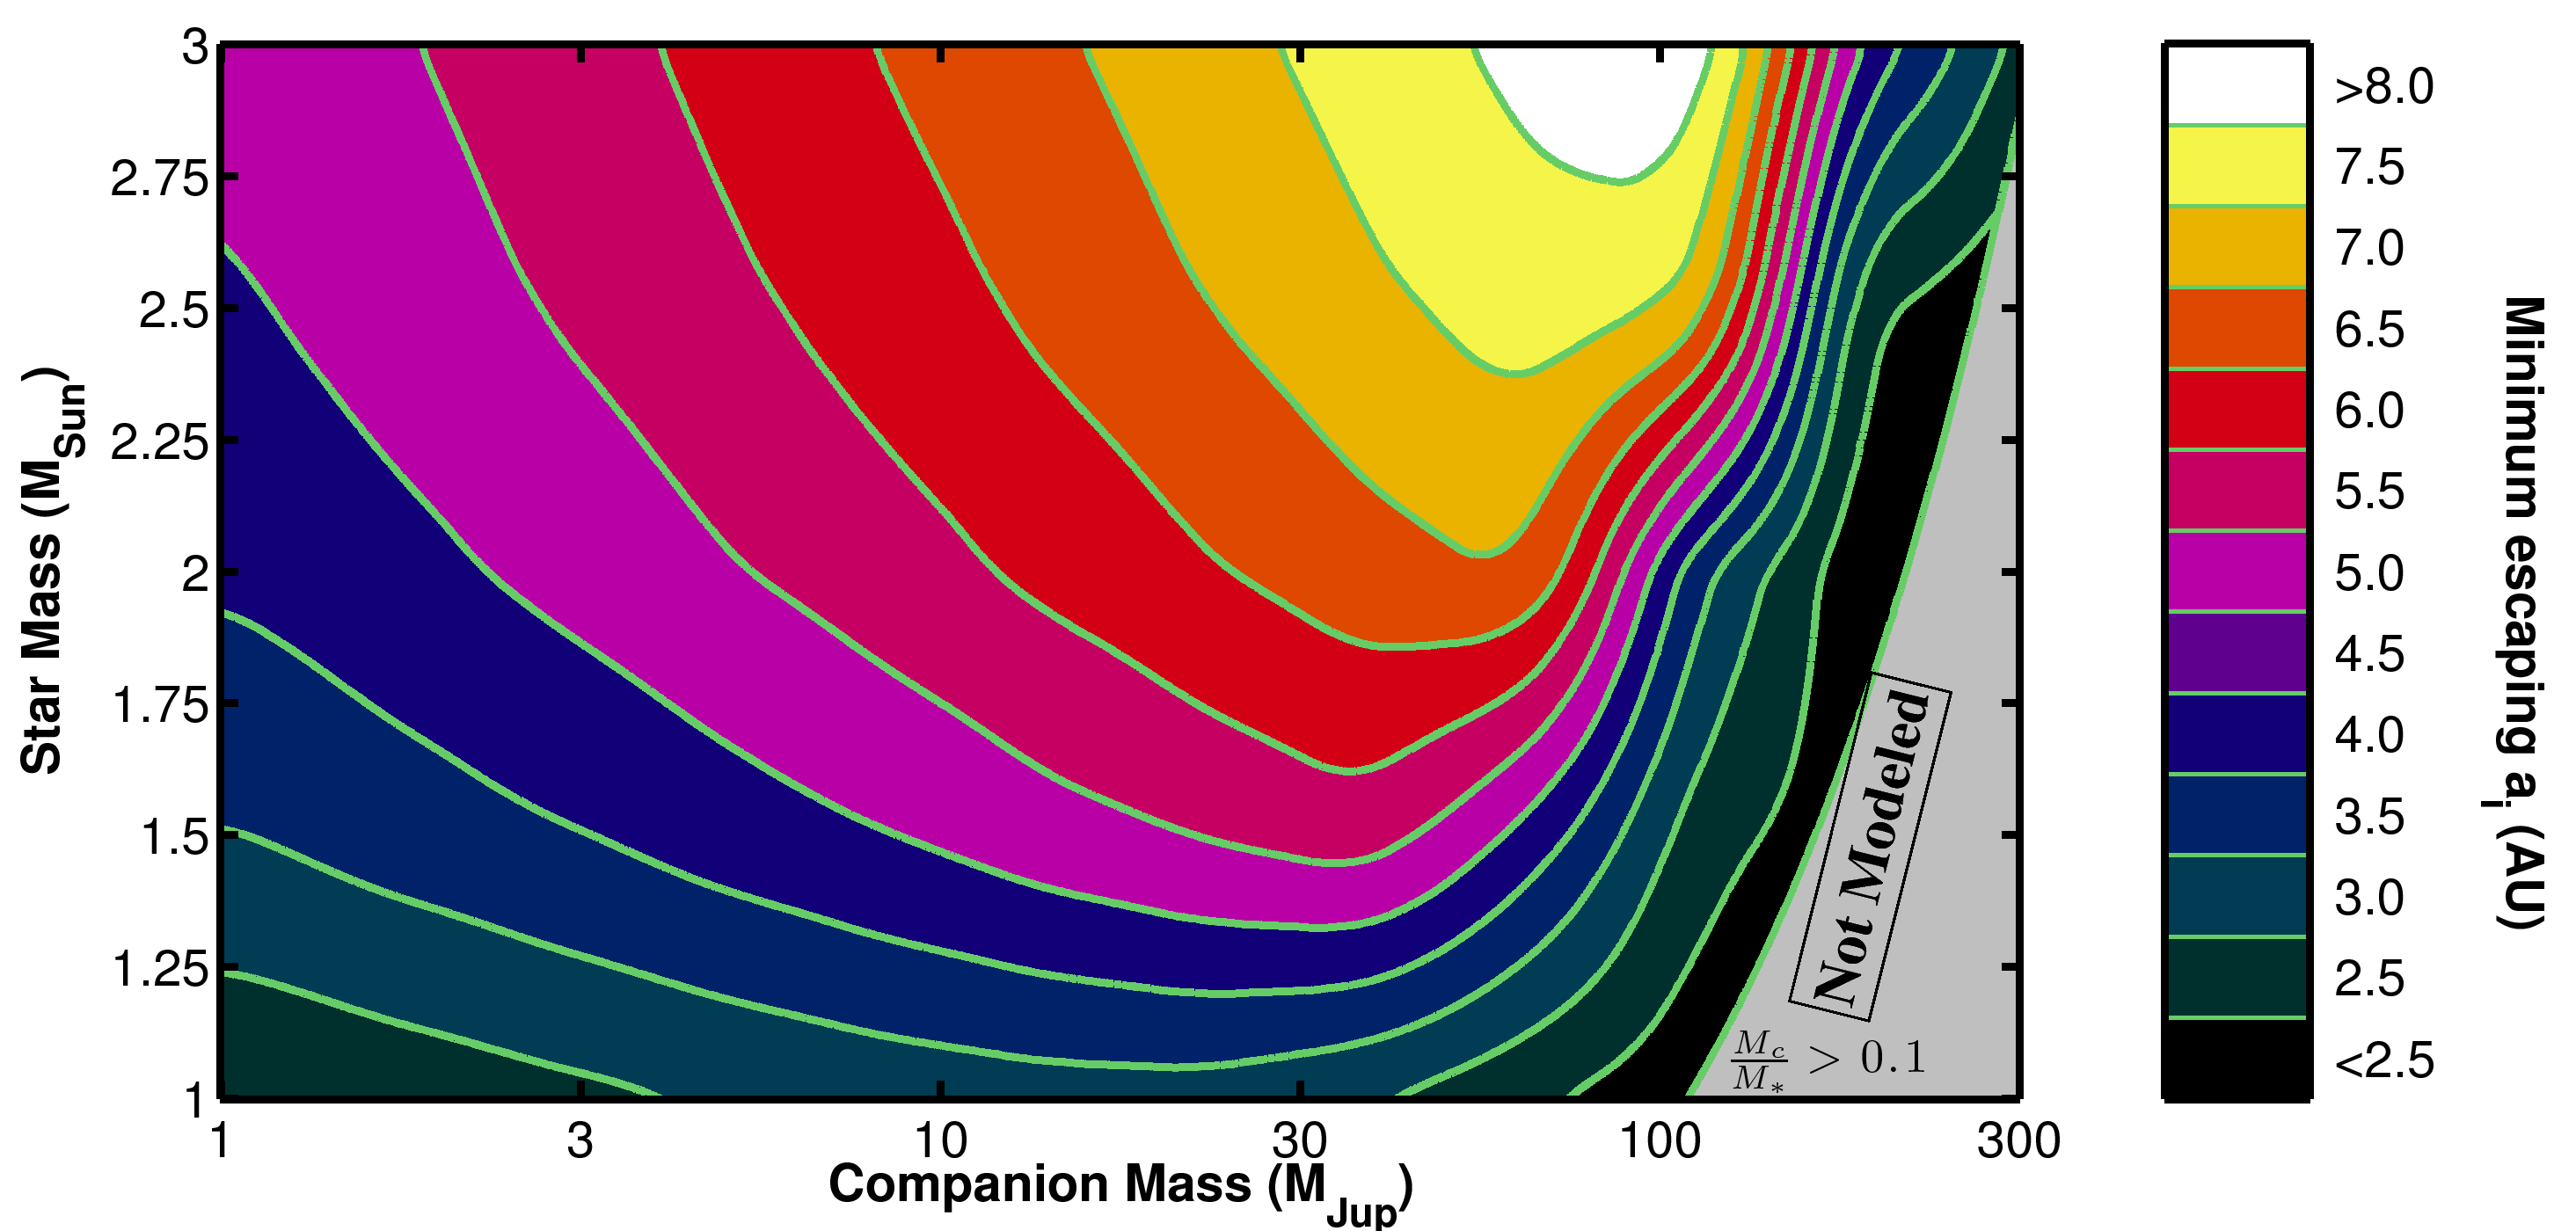
\includegraphics[width=5.4in]{results_fig.png} 
% \vspace*{-1.0 cm}
 \caption{Minimum escaping semi-major axis as a function of companion mass and zero-age main-sequence primary mass under the assumption of quasi-circular orbits (\cite{NS2013}).  Mass ratios greater than 0.1 are not modeled because the primary distorts from spherical symmetry when the companion is near the critical semi-major axis.}
   \label{fig2}
\end{center}
\end{figure}

{\sc\underline{Period Gaps for Companions to White Dwarfs}}: Post-main-sequence evolution naturally produces period gaps for companions to white dwarfs (\cite{2010MNRAS.408..631N, spiegel2012, NS2013}).  At minimum, the expansion of the stellar radius to a few AU would create period gaps by directly engulfing any companion initially orbiting inside this region.  However, giant stars slowly rotate at their surface and possess deep convective envelopes.  An orbiting companion can therefore raise a tidal bulge on the host star such that the orbit decays.  On the other hand, strong, dust-driven winds from the giant act to widen the orbit.  Therefore, for quasi-circular orbits, there exists a critical orbital radius such that companions initially orbiting inside this radius are engulfed and those orbiting outside avoid engulfment (see Figure 1).  Figure 2 shows the minimum escaping semi-major axis ($a_i$) as a function of companion mass and zero-age main-sequence primary mass.  In general, since more massive companions experience stronger tidal torques in proportion to the square of their mass, more massive companions can be tidally engulfed out to a greater initial orbital separation.  However, the contours have an interesting U shape because {\it very} massive companions can tidally synchronize a giant star --- thereby arresting their inspiral --- so to be engulfed they need to begin in a tighter orbit than $\sim$50~$M_{\rm Jupiter}$ comapnions.  The upshot is that massive companions might be found either very close to (orbital period $\lesssim$days) or very far from (orbital period $\gtrsim$years) WDs, while low-mass companions are expected to be found only at large distances from WDs.


{\sc\underline{Formation of Magnetized White Dwarfs}}: Engulfment in a common envelope can lead to one of two outcomes: survival of the companion and emergence in a post-CE orbit, or its destruction (\cite{2006MNRAS.370.2004N}).  The fate of the companion roughly depends on its mass and the binding energy of the envelope at the time of engulfment.  If the companion is of sufficiently low-mass it will not liberate the requisite orbital energy to unbind the envelope and continue migration toward the giant core.  Eventually, the companion will be tidally disrupted as the differential gravitational force due to the proto-WD overcomes the companion's own self-gravity.  For stars possessing low-mass companions such as planets or M dwarfs, there is strong observational evidence that highly-magnetized white dwarfs (with magnetic fields in excess of one MegaGauss, or MG) originate from those systems that destroy the companion in the process.  The tidal disruption of the companion produces a circum-WD accretion disk {\it within} the common envelope (\cite{2011PNAS..108.3135N}).  The disk is initially cold and dense compared to the hot stellar interior.  Magnetic amplification of the initial seed fields via a dynamo can lead to the generation of $>$~MG B-fields which anchor in the proto-WD thereby emerging as a highly-magnetized WD (\cite{2011PNAS..108.3135N}).

\section{Takeaways}
Common envelopes are an important, but poorly understood, phase of stellar evolution.  Observations of outflows in post-AGB/PN have recently lead to an indirect constraint on engine-driving scenarios, namely that accretion in CEs is sufficient to explain all currently observed systems while other scenarios can be ruled out.  Common-envelope phases are also important for stellar evolution as they, along with tidal torques and stellar mass loss, are key ingredients for determining where to look for companions to white dwarfs.  CE systems where the companion is expected to be tidally disrupted inside the common envelope may form accretion disks capable of generating and anchoring strong B-fields in the natal white dwarf.  Such a scenario may explain the origin of highly-magnetized white dwarfs, i.e. those with measured surface fields in excess of 1 MG.  

\begin{thebibliography}{}

\bibitem[Balick \& Frank 2002]{BF2002} Balick, B., \& Frank, A.\ 2002, {\it Ann. Rev. Ast. Astron. Astrophys.}, 40, 439\\

\bibitem[Blackman \& Lucchini (2014)]{BL2014} Blackman, E.~G., \& Lucchini, S.\ 2014, {\it Mon. Not. R. Astron. Soc.}, 440, L16\\

\bibitem[Bujarrabal et al. 2001]{Bujarrabal2001} Bujarrabal, V., Castro-Carrizo, A., Alcolea, J., \& S{\'a}nchez Contreras, C.\ 2001, {\it Astron. Astrophys.}, 377, 868\\

\bibitem[De Marco 2009]{DeMarco2009} De Marco, O.\ 2009, {\it Pub. Astro. Soc. Pacific}, 121, 316\\

\bibitem[Huggins (2012)]{2012IAUS..283..188H} Huggins, P.~J.\ 2012, IAU Symposium, 283, 188\\

\bibitem[Nordhaus \& Blackman 2006]{2006MNRAS.370.2004N} Nordhaus, J., \& Blackman, E.~G.\ 2006, {\it Mon. Not. R. Astron. Soc.}, 370, 2004\\

\bibitem[Nordhaus et al. 2007]{2007MNRAS.376..599N} Nordhaus, J., Blackman, E.~G., \& Frank, A.\ 2007, {\it Mon. Not. R. Astron. Soc.}, 376, 599\\

\bibitem[Nordhaus et al. 2010]{2010MNRAS.408..631N} Nordhaus, J., Spiegel, D.~S., Ibgui, L., Goodman, J., \& Burrows, A.\ 2010, {\it Mon. Not. R. Astron. Soc.}, 408, 631\\

\bibitem[Nordhaus et al. 2011]{2011PNAS..108.3135N} Nordhaus, J., Wellons, S., Spiegel, D.~S., Metzger, B.~D., \& Blackman, E.~G.\ 2011, {\it Proceedings of the National Academy of Science}, 108, 3135\\

\bibitem[Nordhaus \& Spiegel 2013]{NS2013} Nordhaus, J., \& Spiegel, D.~S.\ 2013, {\it Mon. Not. R. Astron. Soc.}, 432, 500\\

\bibitem[Paczynski 1976]{1976IAUS...73...75P} Paczynski, B.\ 1976, Structure and Evolution of Close Binary Systems, 73, 75\\

\bibitem[Spiegel 2012]{spiegel2012} Spiegel, D.~S.\ 2012, arXiv:1208.2276 \\

\bibitem[Zijlstra 2015]{Z2015} Zijlstra, A.~A.\ 2015, {\it Revista Mexicana de Astronomía y Astrofísica}, 51, 221\\

\end{thebibliography}

%\begin{discussion}

%\end{discussion}

\end{document}
